\documentclass{svjour3}\usepackage[]{graphicx}\usepackage[]{color}
%% maxwidth is the original width if it is less than linewidth
%% otherwise use linewidth (to make sure the graphics do not exceed the margin)
\makeatletter
\def\maxwidth{ %
  \ifdim\Gin@nat@width>\linewidth
    \linewidth
  \else
    \Gin@nat@width
  \fi
}
\makeatother

\definecolor{fgcolor}{rgb}{0.345, 0.345, 0.345}
\newcommand{\hlnum}[1]{\textcolor[rgb]{0.686,0.059,0.569}{#1}}%
\newcommand{\hlstr}[1]{\textcolor[rgb]{0.192,0.494,0.8}{#1}}%
\newcommand{\hlcom}[1]{\textcolor[rgb]{0.678,0.584,0.686}{\textit{#1}}}%
\newcommand{\hlopt}[1]{\textcolor[rgb]{0,0,0}{#1}}%
\newcommand{\hlstd}[1]{\textcolor[rgb]{0.345,0.345,0.345}{#1}}%
\newcommand{\hlkwa}[1]{\textcolor[rgb]{0.161,0.373,0.58}{\textbf{#1}}}%
\newcommand{\hlkwb}[1]{\textcolor[rgb]{0.69,0.353,0.396}{#1}}%
\newcommand{\hlkwc}[1]{\textcolor[rgb]{0.333,0.667,0.333}{#1}}%
\newcommand{\hlkwd}[1]{\textcolor[rgb]{0.737,0.353,0.396}{\textbf{#1}}}%

\usepackage{framed}
\makeatletter
\newenvironment{kframe}{%
 \def\at@end@of@kframe{}%
 \ifinner\ifhmode%
  \def\at@end@of@kframe{\end{minipage}}%
  \begin{minipage}{\columnwidth}%
 \fi\fi%
 \def\FrameCommand##1{\hskip\@totalleftmargin \hskip-\fboxsep
 \colorbox{shadecolor}{##1}\hskip-\fboxsep
     % There is no \\@totalrightmargin, so:
     \hskip-\linewidth \hskip-\@totalleftmargin \hskip\columnwidth}%
 \MakeFramed {\advance\hsize-\width
   \@totalleftmargin\z@ \linewidth\hsize
   \@setminipage}}%
 {\par\unskip\endMakeFramed%
 \at@end@of@kframe}
\makeatother

\definecolor{shadecolor}{rgb}{.97, .97, .97}
\definecolor{messagecolor}{rgb}{0, 0, 0}
\definecolor{warningcolor}{rgb}{1, 0, 1}
\definecolor{errorcolor}{rgb}{1, 0, 0}
\newenvironment{knitrout}{}{} % an empty environment to be redefined in TeX

\usepackage{alltt}                     % onecolumn (standard format)
%\documentclass[smallcondensed]{svjour3}     % onecolumn (ditto)
% \documentclass[smallextended]{svjour3}       % onecolumn (second format)
%\documentclass[twocolumn]{svjour3}          % twocolumn

% packages
\smartqed  
\usepackage{mathptmx}  
\usepackage[paperwidth=8.5in,paperheight=11in,top=1in,bottom=1in,left=1in,right=1in]{geometry}
\usepackage{acronym}
\usepackage{hyperref}
\usepackage{cleveref} %after hyperref
\usepackage{titlesec}
\usepackage{multirow}
\usepackage{booktabs}
\usepackage{graphicx}

%acronyms
\acrodef{chl}[chl-\textit{a}]{chlorophyll-\textit{a}}
\acrodef{CV}{coefficient of variation}
\acrodef{ENSO}{El Ni\~{n}o-Southern Oscillation}
\acrodef{EPA}{Environmental Protection Agency}
\acrodef{EPC}{Environmental Protection Commission}
\acrodef{IQR}{interquartile range}
\acrodef{ppt}{parts per thousand}
\acrodef{RMSE}[$RMSE$]{root mean square error}
\acrodef{SST}{Sea Surface Temperature}
\acrodef{TN}{total nitrogen}
\acrodef{WRTDS}{Weighted Regressions on Time, Discharge, and Season}

%cleveref options
\crefname{table}{Table}{Tables}
\crefname{figure}{Fig.}{Figs.}
\renewcommand{\figurename}{Fig.}

% needed to make cleveref play nice with springer template
\makeatletter \let\cl@chapter\relax \makeatother

%assorted functions
%for multiple rows in table headers
\newcommand{\head}[2]{\multicolumn{1}{>{\arraybackslash}p{#1}}{#2}}
%for micrograms per litre
\newcommand{\mugl}{$\mu$g L$^{-1}$}
%90th and 10th percentile models
\newcommand{\nine}{90\textsuperscript{th} percentile }
\newcommand{\ten}{10\textsuperscript{th} percentile }
%for supplemental figures/tables
\newcommand{\beginsupplement}{%
        \setcounter{table}{0}
        \renewcommand{\thetable}{S\arabic{table}}%
        \setcounter{figure}{0}
        \renewcommand{\thefigure}{S\arabic{figure}}%
     }

\journalname{Environmental Modeling and Assessment}

%%%%%%
%knitr stuff
     
%knitr options




%function to format p values


%%%%%%
\IfFileExists{upquote.sty}{\usepackage{upquote}}{}
\begin{document}

\title{Adaptation of a weighted regression approach to evaluate water quality trends in an estuary
}

\titlerunning{Weighted regression for an estuary}        

\author{Marcus W. Beck       \and
        James D. Hagy III
}

\institute{
  M. Beck \at
  ORISE Research Participation Program \\
  USEPA National Health and Environmental Effects Research Laboratory \\
  Gulf Ecology Division, 1 Sabine Island Drive, Gulf Breeze, FL 32561 \\
  Tel.: +18509342480\\
  Fax: +18509342401\\
  \email{beck.marcus@epa.gov}  
  \and
  J. Hagy \at
  USEPA National Health and Environmental Effects Research Laboratory \\
  Gulf Ecology Division, 1 Sabine Island Drive, Gulf Breeze, FL 32561 \\
  Tel.: +18509342455\\
  Fax: +18509342401\\
  \email{hagy.jim@epa.gov}
}

\date{Received: date / Accepted: date}

\maketitle

\begin{abstract}
The increasing availability of long-term monitoring data can improve resolution of temporal and spatial changes in water quality.  In many cases, the fact that changes have occurred is no longer a matter of debate.  However, the relatively simple methods that have been used to evaluate trends in environmental monitoring data in estuaries are often not sufficient to disaggregate the complex effects of multiple environmental drivers, limiting the potential to relate changes to possible causes.  To improve the description of long-term changes in water quality, we adapted a weighted regression approach developed to describe trends in pollutant transport in rivers to analyze a long-term water quality dataset from Tampa Bay, Florida.  The weighted regression approach allows for changes in the relationships between water quality and explanatory variables by using dynamic model parameters and can more clearly resolve the effects of both natural and anthropogenic drivers of ecosystem response.  The model resolved changes in \ac{chl} from 1974 to 2012 at seasonal and multi-annual time scales while considering variation associated with changes in freshwater influence.  Separate models were developed for each of 4 Bay segments to evaluate spatial differences in patterns of long-term change.  Observed trends reflected the known long term decrease in nitrogen loading to Tampa Bay since the 1970s, such that \ac{chl} concentration decreased by 32\% after municipal improvements in wastewater treament. Although trends in mean \ac{chl} have remained constant since mitigation of point-sources of pollution, model predictions indicated that variation has increased in recent years for upper Bay segments, as well as an overall decrease in low productivity events for the lower Bay. Changes in model parameters for the last decade indicated that the relationship of salinity with \ac{chl} was unimodal rather than continuous for upper Bay segments, such that flushing effects were observed beyond specific thresholds.  Results from our analyses have allowed additional insight into water quality changes in Tampa Bay that has not been possible with traditional modeling approaches and the approach could easily be applied to other systems with long-term datasets.
\keywords{Chlorophyll \and Estuary \and Salinity \and Tampa Bay \and Trend evaluation \and Weighted regression}
\end{abstract}

\acresetall
\section{Introduction} \label{intro}

Eutrophication has been documented in aquatic systems worldwide and is of particular concern for coastal waters that support numerous aquatic life and human uses.  Eutrophication is defined as an increase in the rate of supply of organic matter to a system \cite{Nixon95} and is typically caused by elevated nitrogen or phosphorus loads.  Although nutrients are necessary for the growth of primary producers, excessive anthropogenic inputs can have serious consequences for the structure and function of aquatic systems.  Eutrophication of coastal systems has been associated with depletion of dissolved oxygen from the decomposition of organic matter \cite{Diaz08}, increases in the frequency and severity of harmful algal blooms \cite{Glibert13}, and reduction or extirpation of seagrass communities \cite{Duarte95,Tomasko05}.  System-wide changes can occur as the effects of eutrophication on primary production propogate to upper trophic levels \cite{Powers05}. 

The effects of eutrophication are generally well understood, particularly for freshwater systems. The consequences of nutrient pollution were increasingly obvious by the 1960s such that eutrophication became a central focus of limnological research \cite{Cloern01}.  However, the importance of understanding the relative effects of eutrophication on coastal systems were not realized until several decades later.  For example, Rosenberg \cite{Rosenberg85} described the future hazards of coastal eutrophication nearly twenty years after similar issues were the focus of intense study in freshwater systems.  Approaches for describing nutrient dynamics in coastal systems have relied heavily on freshwater eutrophication models that may not adequately describe idiosyncratic behaviors of individual estuaries.  For example, Cloern \cite{Cloern01} suggests that system-specific attributes modulate coastal response to nutrient inputs, such that more appropriate conceptual models that recognize linked changes in relevant state variables are needed.  To date, empirical models that are flexible and appropriate for site-specific conditions have not been extensively applied to describe nutrient-response dynamics in estuaries.

The increasing availability of long-term, high resolution datasets has further underscored the need to develop quantitative nutrient-response models given the potential to extract detailed information on system dynamics.  In many cases \cite{Caffrey03, Greening06}, long-term datasets have sufficiently described general trends in response to changing nutrient regimes or seasonal dynamics, although unambiguous and quantitative descriptions of responses have been lacking.  For example, temporal variations in phytoplankton growth dynamics are often apparent by season with typical late summer blooms in temperate or tropical systems \cite{Cloern96}, whereas climate variation may contribute to substantial deviation in growth patterns between years \cite{Jassby02}.  Additionally, spatial heterogeneity in algal response to nutrients is common across salinity gradients such that effects of flux variation are most apparent near freshwater inflows \cite{Cloern96}.  Simple statistical models that are constrained by assumptions of linearity and stationarity  of variables through time may not adequately characterize subtleties in the variation of nutrient-response measures at different scales.  Novel techniques that leverage the descriptive capabilities of large datasets are needed to improve our understanding of temporal and spatial variation in chlorophyll dynamics as a measure of eutrophication.

Use of simple descriptive statistics to evaluate the effects of water quality management may be ill-advised given that general trends in monitoring data may reflect both management actions and natural variation in system characteristics.  Hirsch et al. \cite{Hirsch10} developed the \ac{WRTDS} approach to model pollutant concentration in rivers to address these issues and shortcomings of previously-developed models.  \ac{WRTDS} enables a flexible interpretation of water quality changes by estimating multiple parameters that are specific to a given season, year, and discharge for individual observations across the time series.  This allows for a more detailed description of water quality changes than standard regression models that characterize trends using a single set of parameters.  Accordingly, the approach addresses the need to focus on descriptions of change in relation to water quality variables across time, rather than hypothesis testing. The approach has been applied to model pollutant delivery from tributary sources to Chesapeake Bay \cite{Hirsch10,Moyer12,Zhang13}, Lake Champlain \cite{Medalie12}, and the Mississippi River \cite{Sprague11}.  The successful applications to water quality trends in rivers suggest the approach could potentially be applied to estuaries to characterize and better understand long-term changes in water quality.  Moreover, changes in pollutant sources and variation in freshwater inputs over time for many coastal systems warrant the use of novel methods for trend evaluation.  Resolving these changes may improve our understanding of linkages between drivers and responses over time. 

Water quality data have been collected in the Tampa Bay estuary (Florida, USA) for approximately forty years.  The natural history of Tampa Bay and the corresponding data provide a useful opportunity for applying quantitative methods to model nutrient dynamics. Nitrogen loads in the mid 1970s were estimated at $8.2 \times 10^6$ kg yr$^{-1}$, with approximately $5.5 \times 10^6$ kg yr$^{-1}$ entering the upper bay alone \cite{Poe05,Greening06}.  Reduced water clarity associated with phytoplankton biomass contributed to dramatic reduction in the areal coverage of seagrass \cite{Tomasko05} and development of hypoxic events causing a decline in benthic faunal production \cite{Santos80}.  Extensive efforts to reduce nutrient loads to the Bay occurred by the late 1970s, with the most notable being improvements in infrastructure for wastewater treatment in 1979.  Improvements in water clarity and decreases in \ac{chl} were observed bay-wide in the 1980s, with conditions generally remaining constant to present day. Although the nutrient management program has been successful in improving water quality, variation in water quality drivers over time suggests the \ac{WRTDS} method could provide information on system dynamics that are not apparent from the observed data.

The goal of the analysis was to describe changes in algal biomass in an estuary in relation to time, season, and freshwater inputs.  We adapted the \ac{WRTDS} approach developed by Hirsch et al. \cite{Hirsch10} to describe water quality trends using a multi-decadal dataset from Tampa Bay, Florida. The analysis addressed four main objectives.  First, we described the weighted regression model and provided a rationale for its adaptation to estuaries.  Second, we applied the model to the time series in different segments of Tampa Bay to characterize trends in both the mean response of \ac{chl} and the frequency of occurrence of extreme events using quantile regression.  Third, additional factors related to water quality were used to describe the unexplained variance in \ac{chl} growth patterns not characterized by the model.  Specifically, model residuals were compared with variation in seagrass growth, \ac{ENSO} effects, and nitrogen load and concentrations in the Bay.  Finally, we developed informed hypotheses to explain temporal and spatial patterns in \ac{chl} growth in response to large scale drivers that affect water quality.  Results from the analysis provide a natural history of water quality changes in Tampa Bay that is temporally consistent with drivers of change.  This analytical approach may improve our understanding of the nutrient-response paradigm in coastal systems.  

\section{Methods}

\subsection{Data}

We compiled a time series of \ac{chl} concentration (\mugl) in Tampa Bay using data from the Hillsborough County \ac{EPC} \cite{TBEP11}.  Data are monthly at mid-depth for each of 50 stations throughout the Bay (\cref{fig:tb_map}) from 1974 to 2012, producing approximately 456 observations per station ($n=$ 1820, \cref{fig:obsyrmo}).  Stations were visited on a rotating schedule such that one third of all stations were sampled each week.  Bay segments represent management units of interest with distinct chemical and physical differences (\cref{tab:segsum}, \cite{Lewis85}).  Accordingly, station data were averaged by segment.  In addition to \ac{chl}, salinity data were obtained and used as a tracer of freshwater influence on water quality.  We expected that salinity was an important factor influencing interpretation of \ac{chl} trends relative to the effects of additional factors (e.g., date, nutrient load, seagrass, etc.).  Salinity data were converted to dimensionless values that represent the fraction of freshwater \cite{Dyer73}, such that:
\begin{equation}
Sal_{ff} = 1 - \frac{Sal_{mea}}{Sal_{ref}}
\end{equation}
\noindent where $Sal_{mea}$ is the measured salinity for a given station and $Sal_{ref}$ is salinity at the seaward reference station for each observation date.  Station 94 in the Gulf (\cref{fig:tb_map}) was used for reference salinity.  Chlorophyll concentrations below the detection limit (censored data) were set to one-half the value from the limit to zero \cite{Gilbert87}.  Chlorophyll data were $ln$-transformed because observations were skewed right, similar to a log-normal distribution.  Kolomogorov-Smirnov tests indicated that the raw data were not signicantly different from theoretical log-normal distributions.

\subsection{Weighted regression}

\ac{WRTDS} was adapted to relate chlorophyll concentration to salinity and time:
\begin{equation}\label{eqn:funform}
\ln\left(Chl\right) = \beta_0 + \beta_1 t + \beta_2 Sal_{ff} + \beta_3 \sin\left(2\pi t\right) + \beta_4 \cos\left(2\pi t\right) + \epsilon
\end{equation}
\noindent where the natural log of \ac{chl} is related to decimal time $t$, salinity $Sal_{ff}$, and unexplained variation $\epsilon$.  Salinity and time are linearly related to \ac{chl} on a sinuisoidal annual time scale (i.e., cylical variation by year). The parameters $\beta_0,\ldots,\beta_4$ are estimated for each observed salinity at time $t$ such that multiple sets of parameters are used to characterize the period of observation.  Decimal time was calculated as the the year and month of each observation as an equivalent decimal (e.g., July 1974 as 1974.5).  Although data were typically not collected on the first of each month, we considered the decimal time coincident with the period of observation.  Additionally, quantile regression models \cite{Cade03} were used to characterize trends at extreme conditional distributions of the data.  Specifically, we adapted the weighted regression approach to model the conditional response at the 10\textsuperscript{th} and 90\textsuperscript{th} quantiles ($\tau=0.1$, and $0.9$, respectively) of the chlorophyll distribution. Quantile regression is analogous to least-squares regression such that a set of $\beta$ parameters that minimizes the error term is estimated, where the minimization function is the sum of the weighted absolute deviations of the fitted values from the observed quantile.  A general interpretation of the fitted values is the distribution of \ac{chl} conditional upon time and salinity for low ($\tau=0.1$) or high ($\tau=0.9$) biomass events, rather than a characterization of `average' conditions using mean models.

The \ac{WRTDS} approach obtains fitted values of the response variable by estimating regression parameters for each unique observation.  Specifically, a regression model was estimated for each of 1,$\ldots$, 456 data points for each Bay segment. Each regression model was weighted by month, year, and salinity such that a unique set of regression parameters for each observation in the time series was obtained. For example, a weighted regression for October 2003 weights other observations in the same year, month, and similar salinity with higher values, whereas observations for different months, years, or salinities receive lower weights (\cref{fig:wtex}).  This weighting approach allows estimation of regression parameters that vary in relation to observed conditions.  Hirsch et al. \cite{Hirsch10} used a tri-cube weighting function:
\begin{equation}
w= \left\{ 
  \begin{array}{l l}
    \left(1-\left(d/h\right)^3\right)^3 & \quad \textrm{if } |d| \leq h \\
    0 & \quad \textrm{if } |d| > h 
  \end{array} \right.
\end{equation}
\noindent where the weight $w$ for each observation is defined by the distance $d$ from the current observation within a window $h$. The weights are diminishing in relation to the current observation until the maximum window width is exceeded and a weight of zero is used.  The weight for each observation is the product of all three weights assigned to month, year, and salinity.  Window widths of six months, 10 years, and half the range of $Sal_{ff}$ for each Bay segment were used (\cref{fig:wtex}).  Window widths were increased by 10\% increments during model estimation until a minimum of 100 observations with non-zero weights were obtained \cite{Hirsch10}.

The adapted \ac{WRTDS} approach was used to model and interpret \ac{chl} trends from 1974--2012 for each of the 4 bay segments.  In contrast with \cite{Hirsch10}, estimates were made using monthly observations rather than daily predictions given the available data for Tampa Bay.  Particular attention was given to trends that have not been previously described.  Following Hirsch et al. \cite{Hirsch10}, predicted values were based on interpolation matrices for each model type (mean, \nine, and \ten) to reduce computation time.  Specifically, a sequence of 20 salinity values based on the minimum and maximum values for each segment were used to predict \ac{chl} using the observed month and year.  Model predictions were then linearly interpolated from the grid using closest salinity value to the actual for each date.  Hirsch et al. \cite{Hirsch10} notes that the introduction of bias associated with using imprecise values in place of actual observations to estimate predictions was minimal.  Model performance was based on coefficients of determination ($R^2$) for the mean regression models and pseudo-$R^2$ values that are specific to given quantiles \cite{Koenker99}.  Additionally, \ac{RMSE} was calculated as an alternative measure of performance such that:
\begin{equation}
RMSE = \sqrt {{\frac{{\sum\limits_{{i = 1}}^n {{{\left( {{y_i} - {{\hat{y}}_i}} \right)}^2}} }}{{n}}}}
\end{equation}
\noindent where $n$ is the number of observations from $1,\ldots,n$ for a given segment, $y_i$ is the observed value of $\ln$-\ac{chl} for observation $i$, and ${\hat{y}}_i$ is the predicted value for of $\ln$-\ac{chl} for observation $i$.  \ac{RMSE} values closer to zero represent model predictions closer to observed. The performance of weighted models were compared to conventional (i.e., non-weighted) additive linear models to show potential improvements using the \ac{WRTDS} approach.   

A potential issue for predictions with regression models in $\ln$-transformed space is bias associated with back-transformation \cite{Duan83}.  Specifically, predicted values that are back-transformed by exponention may be biased due to variation in the concentration-salinity (or concentration-discharge) relationship through changes in residual variation across the data domain.  We followed the approach in Moyer et al. \cite{Moyer12} that corrected for back-transformation bias using a scale parameter that is independently estimated for all regression models in the time series.  The scale parameter describes the variance of the residuals such that: 
\begin{equation}\label{eqn:resvar}
\hat{\sigma}_\epsilon^2 =\frac{\sum\limits_{{i = 1}}^n w_i \left(y_i - \hat{y}_i \right)^2}{\sum\limits_{{i = 1}}^n w_i }
\end{equation}
\noindent where residual variance $\hat{\sigma}_\epsilon^2$ (scale parameter) is the weighted sum of squared errors for chlorophyll for observations $1,\ldots,n$.  Scale parameters were obtained for each unique regression across the time series and used to determine the correction bias in the back-transformation such that:
\begin{equation}\label{eqn:biascorr}
\alpha = \exp\left(\frac{\hat{\sigma}_\epsilon^2}{2}\right)
\end{equation}
\begin{equation}\label{eqn:backtrans}
\hat{Chl} = \alpha \exp\left(\beta_0 + \beta_1 t + \beta_2 Sal_{ff} + \beta_3 \sin\left(2\pi t\right) + \beta_4 \cos\left(2\pi t\right)\right)
\end{equation}
\noindent where the back-transformed chlorophyll concentration $\hat{Chl}$ is the exponentiated model prediction multiplied by the correction factor $\alpha$ \cite{Moyer12}.  Unique scale and correction bias parameters were obtained for each observation that was back-transformed.  Although differences between results from bias-corrected predictions and simple exponentiation were minimal, \cref{eqn:resvar,eqn:biascorr,eqn:backtrans} were used to create more accurate representations of chlorophyll trends in accordance with developed methods \cite{Hirsch10,Moyer12}. 

In addition to trend description, the \ac{WRTDS} approach can be used to normalize predicted values for a given explanatory variable to allow interpretation of trends in the absence of random variation.  For example, water quality trends related to management actions cannot be precisely evaluated if pollutant concentrations vary with discharge.  Hirsch et al. \cite{Hirsch10} used the approach to normalize trends by flow, whereas our adapted approach was used to normalize by salinity which accounts for both freshwater inputs and tidal exchange.  Normalized predictions were obtained for each observation date by assuming that salinity values for the same month in each year were equally likely to occur across the time series.  That is, salinity is assumed to be uniformly distributed within the range of observed values for the same month between years.  For example, normalization for January 1\textsuperscript{st} 1974 considers all salinity values occuring on January 1\textsuperscript{st} for each year in the time series as equally likely to occur on the observed data.  A normalized value for January 1\textsuperscript{st} 1974 is the average of the predicted values using each of the salinity values as input, while holding month and year constant.  Normalization across the time series is repeated for each observation to obtain salinity-normalized predictions.    

\subsection{Evaluation of model residuals}

An advantage of the \ac{WRTDS} approach is the ability to describe water quality trends by considering changes in the relationships among variables for  different observation periods.  Additional factors not related to time or salinity could be used to describe the unexplained variation in the models ($\epsilon$, \cref{eqn:funform}). Residuals for the mean and quantile models in each Bay segment were related to additional variables with considerable management importance: seagrass growth, \ac{ENSO} climate effects by season and year, and nitrogen load and concentrations.  Conventional statistics were used to obtain a general description of the relationships, such as correlation coefficients and linear regression.

Seagrass coverage in Tampa Bay has been estimated bi-annually since 1988 \cite{Tomasko05}.  Coverage data are based on interpretation of aerial photos to produce raster surfaces with pixels coded as continuous ($>$75\%) or patchy (25\%--75\%) coverage.  Areal coverage of seagrass for years with available data ($n=$ 12) were estimated by considering seagrass as present (continous or patchy) or absent within each Bay segment.  \ac{ENSO} data obtained from the Climate Prediction Center \cite{CPC13} were based on a three year running-average of \ac{SST} anamolies in the Ni\~{n}o 3.4 region of the Pacific Ocean (5$^{\circ}$N--5$^{\circ}$S, 120$^{\circ}$--170$^{\circ}$W).  \ac{SST} index values greater (less) than 0.4 (-0.4) were considered El Ni\~{n}o (La Ni\~{n}a) conditions, neutral otherwise.  \ac{SST} index values were categorically and quantitatively summarized by year and season using designations in Lipp et al. \cite{Lipp01}: winter - January, February, March; spring - April, May, June; summer - July, August, September; fall - October, November, December.  Finally, monthly loads for \aclu{TN} (\acs{TN}, kg/mo) from 1985--2007 were obtained \cite{Zarbock94,Pribble01,Poe05}, in addition to \ac{TN} concentration from monitoring data \cite{TBEP11}.  Nitrogen loads are based on estimated and measured contributions from nonpoint sources, point sources, atmospheric deposition, groundwater, and losses of phosphate rock and fertilizer from industrial processes.

%\begin{acknowledgements}
%If you'd like to thank anyone, place your comments here
%and remove the percent signs.
%\end{acknowledgements}

% BibTeX users please use one of
% \bibliographystyle{spbasic}      % basic style, author-year citations
\bibliographystyle{spmpsci}      % mathematics and physical sciences
% \bibliographystyle{spphys}       % APS-like style for physics
\bibliography{M:/docs/ref_diss}   % name your BibTeX data base

%%%%%%
%tables

%segment characteristics
% latex.default(dat, file = "", caption.loc = "top", caption = cap.val,      insert.bottom = foot.val, rowname = segs, colheads = cnames,      rowlabel = "Segment", label = "tab:segsum", digits = 5, double.slash = F,      multicol = F, col.just = rep("l", ncol(dat))) 
%
\begin{table}[!tbp]
\caption{Summary of characteristics for Tampa Bay segments.  Mean chlorophyll and salinity data for 2012 are shown. Sources: \cite{Lewis85,Lewis88}.\label{tab:segsum}} 
\begin{center}
\begin{tabular}{lllllll}
\hline\hline
Segment&\head{2cm}{Area (km$^2$)}&\head{2cm}{Shoreline length (km)}&\head{2cm}{Mean depth (m)}&\head{2cm}{Watershed area (km$^2$)}&\head{2cm}{Chlorophyll-\textit{a} (\mugl)}&\head{2cm}{Salinity}\tabularnewline
\hline
HB&$105.3$&$128.6$&$3.2$&$3319.9$&$9.9$&$24.4$\tabularnewline
OTB&$200.7$&$339.8$&$2.8$&$ 874.4$&$7.6$&$23.5$\tabularnewline
MTB&$309.9$&$262.8$&$4.1$&$1062.7$&$6.1$&$27.1$\tabularnewline
LTB&$246.6$&$121.6$&$3.8$&$ 330.5$&$4.1$&$32.2$\tabularnewline
\hline
\end{tabular}
\end{center}
\footnotesize \textit{Note:} HB: Hillsborough Bay, OTB: Old Tampa Bay,  MTB: Middle Tampa Bay, LTB: Lower Tampa Bay\end{table}



%%%%%%
%figures

%map of TB, made in ArcMap
\begin{figure}
\centering
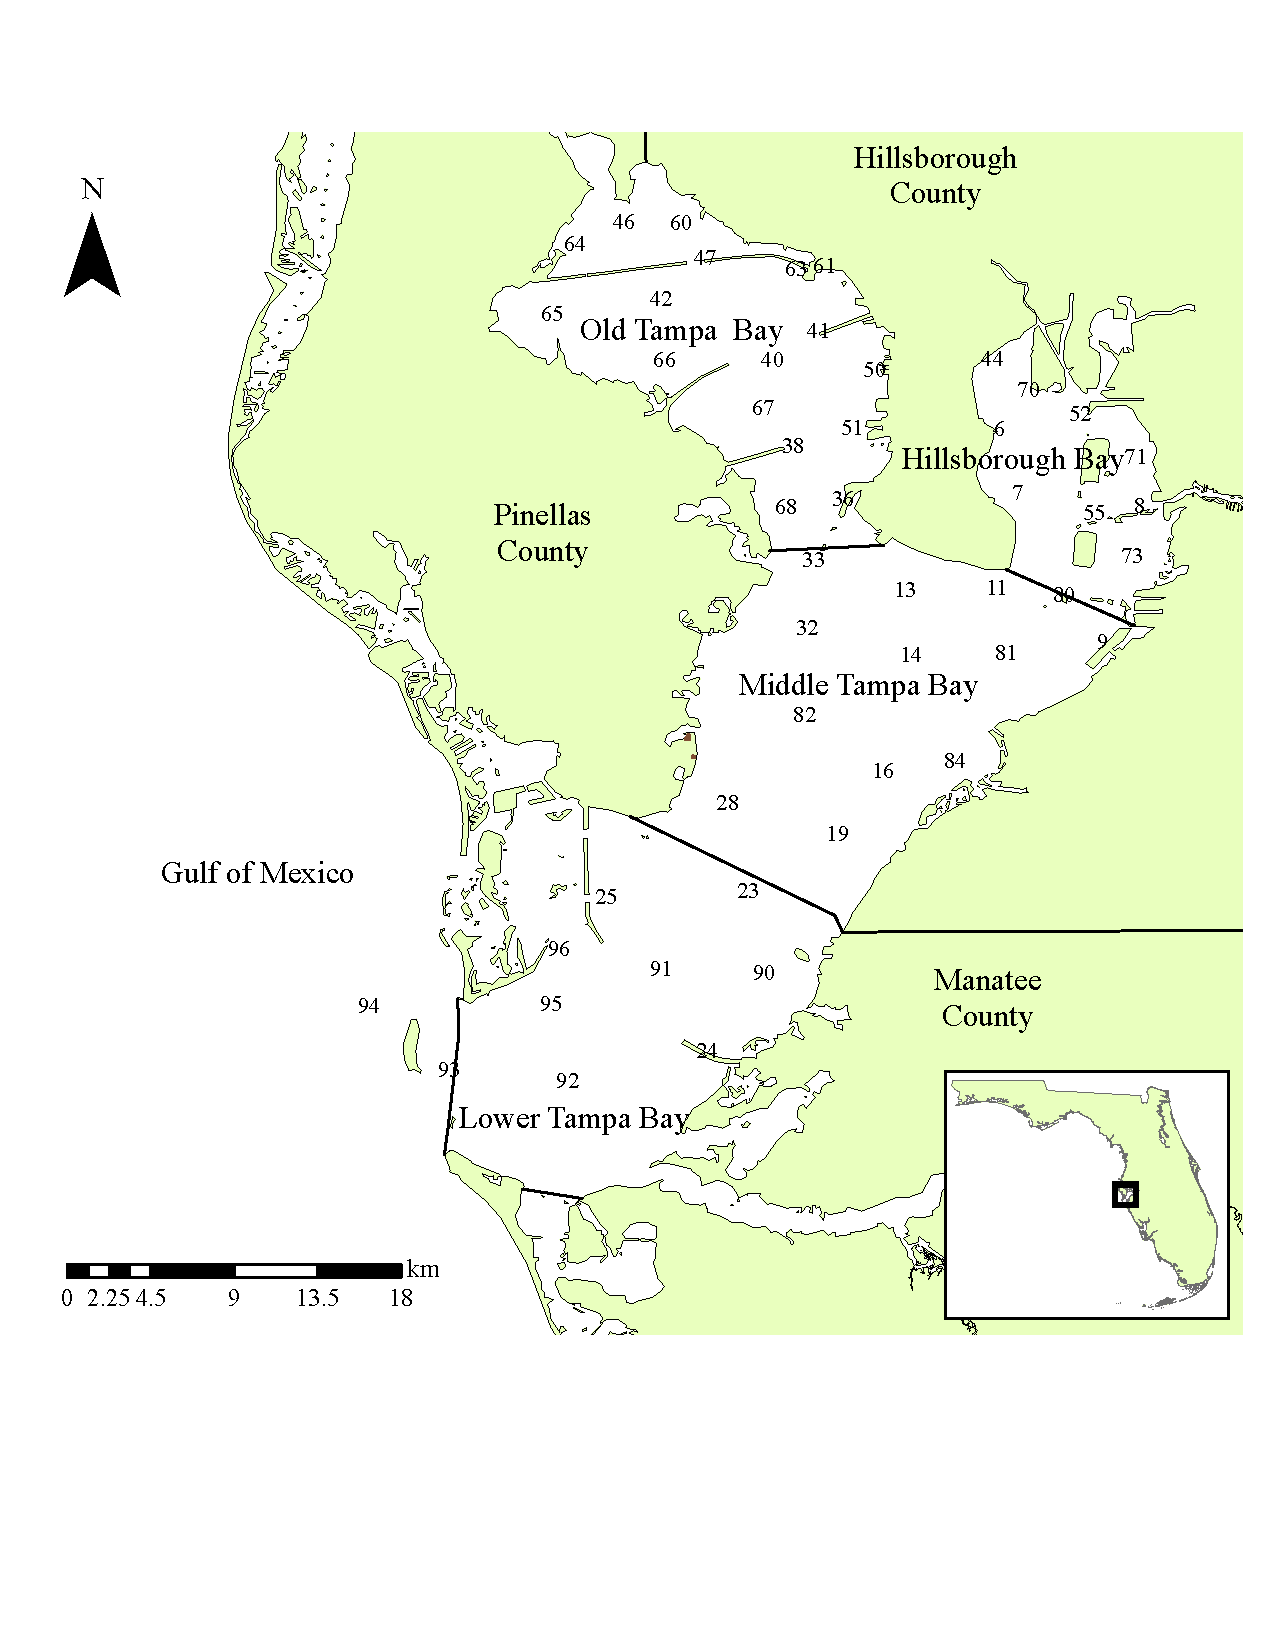
\includegraphics[width=0.9\textwidth]{M:/docs/manuscripts/tb_chl/figs/tb_map.pdf}
\caption{The Tampa Bay estuary located on the west coast of central Florida. The Bay is separated into four segments defined by chemical, physical, and geopolitical boundaries \cite{Lewis85}. Monthly water quality monitoring stations are also indicated by their identification number \cite{Boler01}.}
\label{fig:tb_map}
\end{figure}

%obs chlorophyll by year/month, uses station data

\begin{figure}
\centering
\subfloat[By year]{
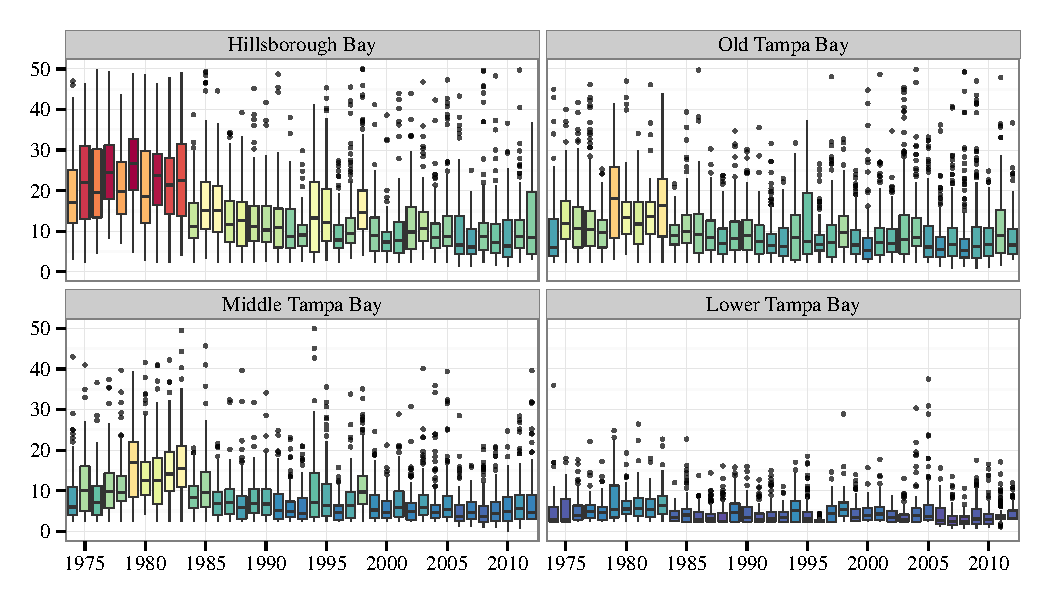
\includegraphics[width=\textwidth,page=1]{M:/docs/manuscripts/tb_chl/figs/obsyrmo.pdf}
\label{fig:obsyrmo1}
}

\subfloat[By month]{
\includegraphics[width=\textwidth,page=2]{M:/docs/manuscripts/tb_chl/figs/obsyrmo.pdf}
\label{fig:obsyrmo2}
}

\leavevmode\smash{\makebox[0pt]{\hspace{0em}% HORIZONTAL POSITION           
  \rotatebox[origin=l]{90}{\hspace{19em}% VERTICAL POSITION
    Chlorophyll-\textit{a} (\mugl)}%
}}\hspace{0pt plus 1filll}\null

\caption{Observed \ac{chl} data for Tampa Bay segments by \protect\subref{fig:obsyrmo1} year and \protect\subref{fig:obsyrmo2} month aggregations.  Each box is bisected by the median and represents the \ac{IQR} (25\textsuperscript{th} to 75\textsuperscript{th} percentile).  Outliers are present beyond whiskers (1.5$\cdot$\ac{IQR}) and were observed beyond 50 \mugl.  HB: Hillsborough Bay, MTB: Middle Tampa Bay, OTB: Old Tampa Bay, LTB: Lower Tampa Bay.}
\label{fig:obsyrmo}
\end{figure}

\end{document}
% end of file template.tex
